\begin{figure}[h]
    \centering
    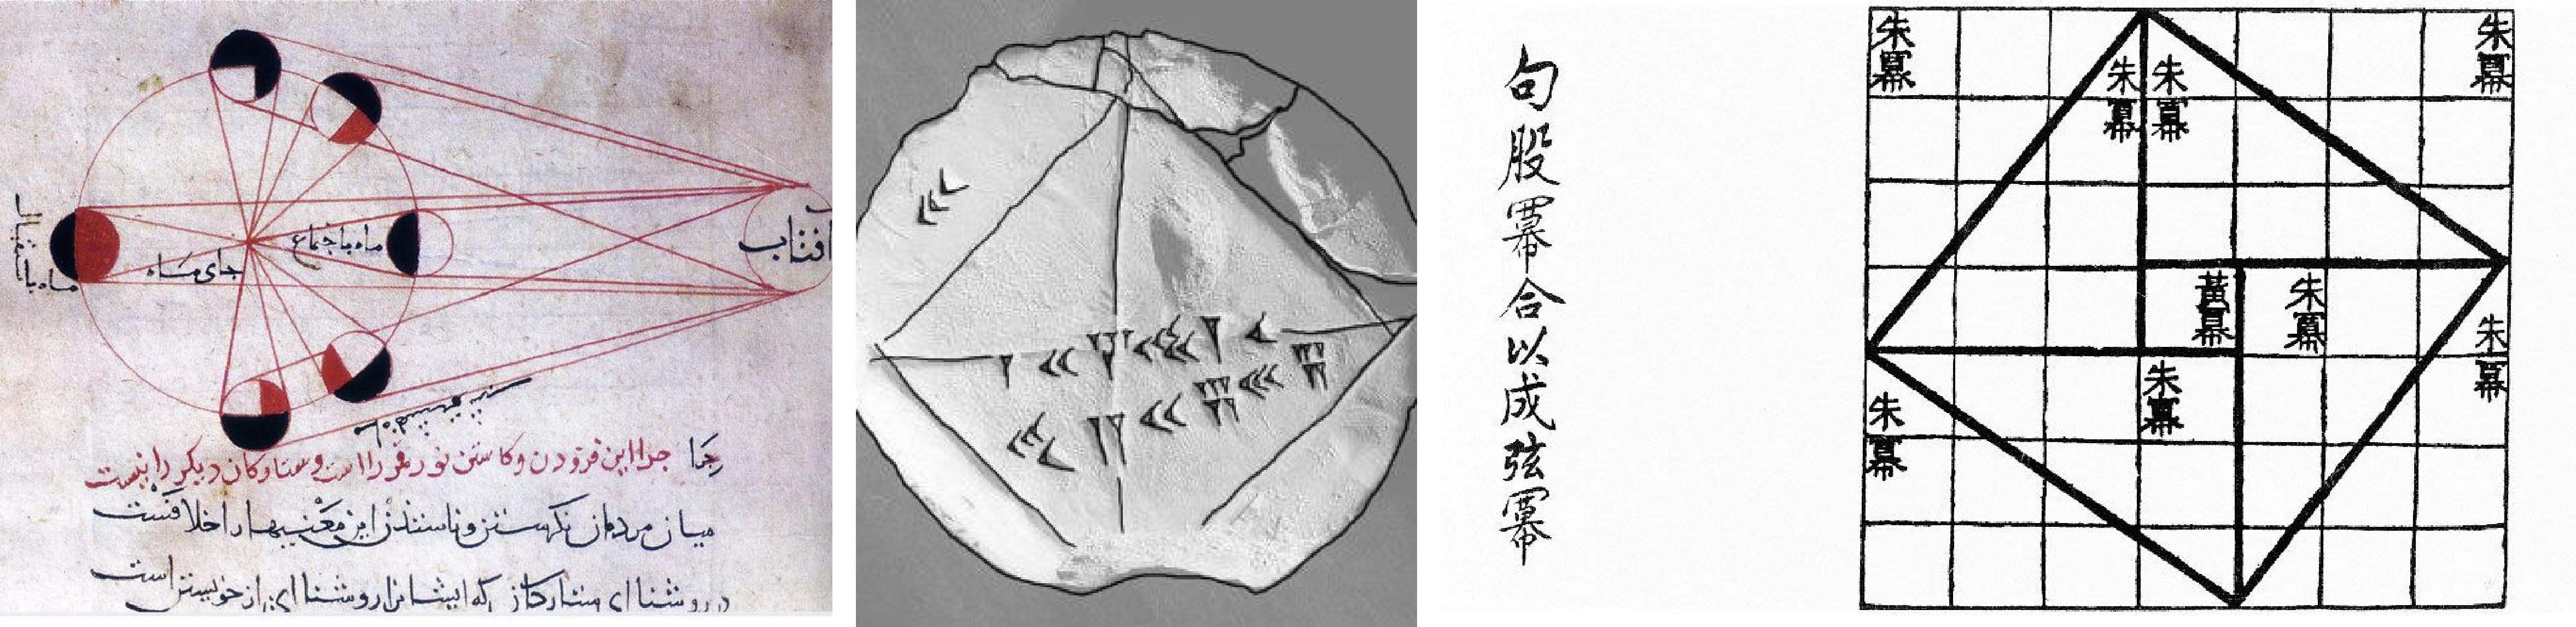
\includegraphics[width=\linewidth]{assets/related-work/historical-diagrams.pdf}
    \caption{Several examples of ancient diagrams, from left to right: (1) Phases of the Moon: Abu Rayhan Muhammad ibn Ahmad al-Biruni (Iranian, 973-1048), (2) Babylonian clay tablet diagramming an approximation of $\sqrt{2}$ (1900 -1700 BCE), and (3) Geometric proof of the Pythagorean theorem in Zhoubi Suanjing 周髀算经 (1st century BCE).}
    \label{fig:ancient-diagrams}
\end{figure}

This chapter provides background on diagrams in general, existing diagramming tools, and research on using diagrams for learning.

\section{Diagrams}
\label{sec:diagrams}

\citet{tversky_diagrams_2017,tversky_visualizing_2011} defines diagrams as \quotei{an arrangement of marks on a virtual page (stone, paper, or screen) that represents a set of ideas and their relations}. This definition is broad enough to include many ancient and modern graphical representations of ideas, including graphs, charts, infographics, and many more. Under this definition, diagrams are perhaps one of the oldest form of human communication and expression. For instance, \cref{fig:ancient-diagrams} shows a few examples of diagrams in ancient times around the world. Although there are many more definitions of diagrams (for example, \cite{bender_culture_2010,card_readings_1999,infographics,arnheim_visual_1969,tufte1983visual}), this chapter does not aim to provide a comprehensive discussion of how diagrams are defined. Rather, we examine two aspects of a diagram to motivate the types of graphics this dissertation focuses on: content and utility.

First, this dissertation contribute tools (\cref{chp:penrose,chp:edgeworth}) that produce diagrams that depict logical, non-quantitative \textit{concepts}, rather than quantitative \textit{data}. As we will discuss in \cref{sec:related-systems,chp:interviews}, this focus on conceptual diagrams is largely driven by the relative dearth of tools for making conceptual diagrams. In contrast, statistical graphics~\cite{wilkinson_grammar_2012} largely depict quantitative data, and are well supported by authoring tools~\cite{d3, vega}. 

The second aspect is the utility of diagrams, which set them apart from decorative paintings, photos, floor plans, and more. \citet{designWithDiagrams} distinguishes between \emph{pictorial} and \emph{propositional} graphics: instead of directly visualizing data or depicting naturalistic scenes, diagrams (propositional graphics in \citeauthor{designWithDiagrams}'s terms) ``constitute knowledge and embody media-independent abstractions for inference-making.'' The specific utility of diagrams for inference-making is significant enough to prompt psychologists and cognitive scientists to study their role in problem-solving and learning. Diagrams have been shown to have cognitive benefits to reasoning and problem-solving~\cite{whyDiagramWorth, koedinger_emergent_1992, mayer_multimedia_2002}. Compared to textual representations, diagrams facilitate fast recognition and direct inference by making the most relevant information explicit and easily findable~\cite{whyDiagramWorth}. As an external representation of abstract structures of tasks, diagrams can work together with one's mental representation and are an indispensable part for accomplishing distributed cognitive tasks~\cite{DistributedCognitive}. Akin to \citet{designingWithDiagrams}, \citet{hegarty_types_1999} distinguish between \emph{pictorial} and \emph{schematic} visual representations and show that schematic representations of relative spatial relationships significantly outperform pictorial ones that encode visual appearances.
In addition to their values as an external, static representation of knowledge, diagrams are also beneficial when people learn \emph{with}, instead of \emph{from} them~\cite{tippett_what_2016}. In educational contexts, explicit training of drawing, including the creation of new visual representations and adoption of new ones, significantly improve students' ability to work with multiple representations and improve learning, reasoning, and communication skills~\cite{ainsworth_drawing_2011}. Moreover, creating diagrams as visual explanations also improves learning, since they can act as a check for completeness and a medium for inference~\cite{bobek_creating_2016}. 

% In general, people do not need formal training in visual design to create and interpret effective diagrams and learners at all levels can benefit tremendously from creating diagrams~\cite{ABC}.

Beyond diagrams' utility for more efficient cognitive inference and learning, logicians, mathematicians, and philosophers have argued for diagrams' fundamental role in reasoning. Historically, diagrams were often dismissed as mere illustrations---supplementary tools rather than central components of logical arguments. This traditional view has been predominantly influenced by the dominance of symbolic languages in the history of logic, where precision and formal rigor were prioritized over visual representation~\cite{shin_diagrams_2018}. Peirce's existential graphs~\cite{peirce_collected_1931} are a form of diagrammatic logic that he argued could represent logical relations in a manner both clearer and more intuitive than traditional symbolic logic. Peirce believed that existential graphs could express logical relationships with a degree of generality and precision that rivals, if not surpasses, that of symbolic logic, particularly in their ability to represent the continuity of logical processes. Jon Barwise and John Etchemendy's work on the importance of diagrams in logical reasoning~\cite{barwise_visual_2019} aligns closely with the earlier insights of Peirce. Peirce's existential graphs, which visually represent logical propositions and their relationships, serve as a precursor to Barwise's concept of ``heterogeneous reasoning,''~\cite{barwise_heterogeneous_1993} where visual and symbolic methods are integrated to solve logical problems more effectively. 


% In addition to knowledge representation, conceptual diagrams are also a medium for creativity and exploration, since they do not require early commitments to design decisions and focus on the \emph{form} of possible solutions~\cite{ConceptualArchDesign}.

% TODO: diagrams generate information

% \subsection{Cognitive benefits of diagrams for learning and problem-solving}
% \label{sec:diagram-benefits}

\section{Learning how to use diagrams}


Whether for more efficient problem-solving or logical reasoning, one must learn how to use diagrams properly. At the end of \citetitle{whyDiagramWorth}, \citet{whyDiagramWorth} noted that:

\begin{quote}
[D]iagrams are useful only to those who know the appropriate computational processes for taking advantage of them. Furthermore, a problem solver often also needs the knowledge of how to construct a ``good'' diagram that lets him take advantage of the virtues [of diagrams] we discussed.~\cite[p.~99]{whyDiagramWorth}
\end{quote}

In this section, we provide background on why students need to practice for better fluency in visual representations and how diagram variations may help students practice using them more effectively. 

\subsection{Representational fluency and contrasting cases}

Representational fluency refers to the ability to quickly understand a visual representation and to use it to solve domain-specific tasks~\cite{multipleReps}. To become representationally fluent, an important first step is to identify meaningful aspects of a particular representation. \citet{kellman_perceptual_2010} show that mapping between symbolic and visual representations leads to intuitions about the way equivalent structures relate to each other. The learning that results from constructing connections between symbols and diagrams can be more flexible. Students are better at transferring their learning from the problems they have explicitly practiced to more open-ended problems and their conceptual understanding is better~\cite{25learning}. 

In addition to mapping between representations, \citet{marton_sameness_2006} also showed that contrasting cases help students discern crucial parts of a particular representation. Early on, students benefit from discerning instances and noninstances that differ in only one dimension of variation. As students become more fluent, a \emph{fusion} of multiple varying dimensions in problems may be necessary~\cite{chik_simultaneity_2004}. \citet{arnheim_visual_1969} characterized this need for many diagrams (or animation of diagrams) in \citetitle{arnheim_visual_1969}:

\begin{quote}
The usual illustrations in textbooks and on the blackboard help to make a problem visible, but they also freeze it at one phase of the range to which the proposition refers. Therefore, they tempt the student to mistake accidental circumstances for essential ones. The solution is not to leave out illustrations but either to produce mobile models\dots{} or, at least, to use immobile illustrations in such a way that the student realizes which of their dimensions are variables. ~\cite[p. 182]{arnheim_visual_1969}
\end{quote}

\subsection{Multiplicity of examples}

Indeed, in addition to training representational fluency, multiple examples and repeated, varied practice are well-documented strategies for broader learning goals in the learning science literature. Many studies have demonstrated substantial science, technology, engineering, and mathematics (STEM) learning benefits for multiple worked examples per topic \cite{pashler_organizing_2007}. Equally important is research indicating the importance of active learning \cite{chi_icap_2014,deslauriers_measuring_2019} and repeated practice \cite{deliberatePractice,schnackenberg_learner_1998} that occurs within varied contexts \cite{PV94,rohrer_shuffling_2007} and involves direct explanatory feedback \cite{kellman_perceptual_2010}.

\citet{rau_conditions_2017} reports that, unfortunately, providing computational support for representational fluency is time-consuming with current tools. Our formative study (\cref{sec:edgeworth-formative}) confirmed this claim and revealed barriers resulting from the limitations of diagram authoring tools. To address these limitations, \Edgeworth (\cref{chp:edgeworth,chp:edgeworth-eval}) aims to simplify the workflow for creating diagram variations for repeated practice. 


\section{Digital diagramming tools}
\label{sec:related-systems}

% Intro
As this dissertation investigates diagram authoring empirically (\cref{chp:interviews}) and contributes a new diagramming tool (\Penrose, \cref{chp:penrose}), we survey existing digital tools for making diagrams. Although many diagramming tools support both text-based and graphical interfaces, we categorize current diagramming tools by their dominant mode of interaction: programming-language based (PL) tools and direct manipulation (DM) tools. 

% Programming languages: DSL, general purpose
We use PL tools to refer to text-based diagramming tools, including imperative or declarative programming languages, libraries, frameworks, and embedded domain-specific languages. General-purpose tools such as Processing~\cite{Reas:2006:PPM}, Asymtote~\cite{Bowman:2008:AVG}, PGF/TikZ, and Paper.js\footnote{\url{http://paperjs.org/}} provide program constructs that model graphical primitives and operations akin to those in Scalable Vector Graphics (SVG)~\cite{SVGStandard}. Many of their shared disadvantages are well summarized in TikZ's manual~\cite{TikZ-Manual}: ``steep learning curve, no WYSIWYG, small changes require a long recompilation time, and the code does not really ``show'' how things will look like.'' Domain-specific tools allow diagram specifications that are higher-level and specialized to the problem domain to smoothen the learning curve. They are developed either from scratch (\eg~GraphViz and the DOT language for graph visualization~\cite{Graphviz}) or on top of general-purpose tools (\eg~TikZ's extensions, \texttt{tkz-euclide} for Euclidean geometry). However, many of them still inherit the other disadvantages from above. 

DM tools represent interactive diagramming tools that support WYSIWYG interfaces and direct interaction with shapes. Akin to PL tools, general-purpose DM tools such as Adobe Illustrator, Inkscape, and Figma also have similar sets of primitives, but often provide a large number of widgets or drawing tools (\eg~Illustrator CC has nearly 100 built-in tools\footnote{\url{https://helpx.adobe.com/illustrator/user-guide.html}}). To overcome the disadvantage of their highly manual interaction model, both Illustrator and Inkscape provide language bindings or command-line tools for automation, but they still suffer from the above problems of PL tools. Popular domain-specific diagramming tools such as draw.io and Gliffy are template editors that provide predefined, mostly box-and-arrow style shapes, limiting users to a narrow set of diagrams. Research prototypes such as Sketchpad~\cite{sketchpad} and ThingLab~\cite{thinglab} automate diagram layout using constraint solving, but many edit actions like selection and shape construction remain manual. Other prototypes like Apparatus\footnote{\url{http://aprt.us/}} and Bret Victor's dynamic visualization tool~\cite{dynamicViz} incorporate some limited programmatic operations (\eg~macro recording, variable declaration, and computed properties) via direct interactions. 

% 3 Wave of data visualization: the point is, diagramming tools haven't caught up with the dataviz trend
% Statement of our goals
As discussed by \citet{satyanarayan_critical_2020}, data visualization tools have transformed over the past decade. The major advances are characterized by three ``waves'': (1) improvement of individual charts' quality, (2) theories and tools that enable mass-production of visualizations, and (3) the convergence of tools~\cite{thirdWaveViz}. Whereas the benefits of conceptual diagrams are clear and theoretical foundations exist, most of the diagramming tools are still not easily scalable and there are large gaps in existing technologies, notably between PL and DM tools. In other words, the \nth{2} wave of conceptual diagramming is still not here. In the interview study presented in \cref{chp:interviews}, we aim to gain a deep understanding of people's diagramming process to drive the design of tools that fill these gaps.



% \subsection{Empirical studies on diagramming-related activities}

% Although conceptual diagrams are widely studied as a powerful visual representation in multiple domains, there has not been a significant amount of prior work that focuses on the \emph{authoring} of conceptual diagrams, especially with digital tools. 

% However, prior work in related activities such as note-taking and whiteboarding suggests some insights for both understanding these activities and opportunities for tool design. Studies on sketches in STEM~\cite{Whiteboards} and software engineering~\cite{Whiteboards-Ko} suggest a need for automating the process of sketching and preserving transient sketches such as whiteboard drawings with appropriate tools. In similar activities such as annotating documents, personal annotations undergo dramatic changes such as significant substantiation and clarification when they are shared on public platforms~\cite{Annotations}. Digitization of the analog pen-and-paper interface attempts to make the transformation process smoother. While digital ink tools imitate the pen-and-paper experience and provide more versatility and power, there still exist gaps between the manual and digital experience of sketching due to conflicting affordances of analog pen and digital ink~\cite{AsWeMayInk}. 

% Given the lack on the prior work on this topic, \cref{chp:interviews} directly investigates the process of creating conceptual diagrams using digital tools.

 

% %%%%%%%%%%%%%%%%%%%%%%%%%%%%%%%%%%%%%%%%%%%%%%%%%%%%%%%%%%%%%%%%%%%%%%%%%%%%%%%% Not used


% % User-centered design is good
% % Recent research demonstrated significant usability and efficiency gains when empirical data are used to motivate tool design. For instance, Playful Palette~\cite{PlayfulPalette} addresses visual artists' needs elicited from a pilot user study and showed effectiveness by increasing the usage of distinct colors by 39\% and amplifying artists' creativity. The design of Data Illustrator was informed by intensive interviews with graphic designers and the result was a tool that enhanced users abilities to compose visualizations~\cite{DataIllustrator}. Our goal in this paper is to study the process of creating conceptual diagrams to drive the design of tools that support this process. 


% % \subsection{Empirical studies on diagramming-related activities}

% % \todoi{go through this section again and consider removing it}

% % Empirical studies on diagramming and related domains have revealed cognitive and behavioral patterns of how people interact with external representations such as diagrams and notes. These findings inform our study of how domain experts create conceptual diagrams.

% % Grammel \etal{} found that, When making information visualizations, novices tend to operate on higher-level constructs in both the data and visual spaces: they prefer to operate on their high-level mental models of the data rather than data attributes; they also tend to use composite visual constructs (\eg~bars and tree nodes) rather than primitives (\eg~polygons and circles)~\cite{NoviceInfoviz}. 

% % % Do domain experts, who have a better grasp of the semantic meaning of data, use similar generic visual constructs? In this study, we investigate how conceptual diagrammer find and construct high-level representations to aid their thinking. 

% % Studies on sketches in STEM~\cite{Whiteboards} and software engineering~\cite{Whiteboards-Ko} suggest a need for automating the process of sketching and preserving transient sketches such as whiteboard drawings with appropriate tools. In similar activities such as annotating documents, personal annotations undergo dramatic changes such as significant substantiation and clarification when they are shared on public platforms~\cite{Annotations}. Digitization of the analog pen-and-paper interface attempts to make the transformation process smoother. While digital ink tools imitate the pen-and-paper experience and provide more versatility and power, there still exist gaps between the manual and digital experience of sketching due to conflicting affordances of analog pen and digital ink~\cite{AsWeMayInk}. In this paper, we investigate the process of transforming sketches to digital, formal versions. 

% % Penrose

% \subsection{Diagramming Systems}
% \label{sec:RelatedSystems}

% Here we consider how our system design relates to other systems that convert abstract mathematical ideas into visual diagrams.  Other classes of tools, such as general-purpose drawing tools (\eg{}, \emph{Adobe Illustrator}) can also be used to make diagrams, though one quickly runs into barriers, such as for large-scale diagram generation or evolving the style of a large collection of existing diagrams.  A broader discussion of related work can be found in a pilot study we did on how people use diagramming tools~\cite{Ni:2020:HDE}.

% There are three main kinds of systems that convert an abstract form of input (\eg{}, an equation or code) into a visual representation.  Language-based systems, such as \textit{TikZ}~\cite{TikZ-Manual} (which builds on \TeX), are domain-agnostic and provide significant flexibility for the visual representation. Their use of ``math-like'' languages influenced the design of \Substance.  However, existing systems do not aim to separate mathematical content from visual representation. For instance, TikZ is domain- and representation-agnostic because it requires diagrams to be specified at a low level (\eg{}, individual coordinates and styles) making programs hard to modify or reuse.  Moreover, since there are only shallow mathematical semantics, it becomes hard to reason about programs at a domain level.

% Plotting-based systems, like \emph{Mathematica} and \emph{GeoGebra}~\cite{geogebra5} enable standard mathematical expressions to be used as input and automatically generate attractive diagrams.  Just as a graphing calculator is easy to pick up and use for most students of mathematics, these tools inspired us to provide a ``tiered'' approach to \Penrose{} that makes it accessible to users with less expertise in illustration (\figref{NoviceExpertUsers}). However, much like a graphing calculator, the visual representations in these systems are largely ``canned,'' and the set of easily accessible domains is largely fixed.  For instance, \emph{Mathematica} does not permit user-defined types, and to go beyond system-provided visualization tools, one must provide low-level directives (in the same spirit as tools like \textit{TikZ}).

% Finally, systems like \emph{graphviz}~\cite{Graphviz}, and \emph{Geometry Constructions Language}~\cite{Janivcic:2006:GCLC} translate familiar domain-specific language into high-quality diagrams. Here again, the domains are fairly narrow and there is little to no opportunity to expand the language or define new visualizations.  Yet the convenience and power of such systems for their individual domains inspired us to build a system with greater extensibility. More broadly, while all these systems share some design goals with ours, a key distinction is that \Penrose\ is designed from the ground up as an extensible \emph{platform} for building diagramming tools, rather than a monolithic end-user tool.


% % Edgeworth


% \section{Background and Related Work}


\section{Tools for Problem Generation}
\label{sec:problem-generation}

In addition to making standalone diagrams, this dissertation also covers diagrammatic problem authoring with \Edgeworth in~\cref{chp:edgeworth,chp:edgeworth-eval}. In this section, we cover related digital systems for practice problem generation in general, and their support for diagram authoring. \citet{kurdi_systematic_2020} conduct a systematic review of automatic problem generation tools and show that the majority of tools address language learning. In this section, we focus on problem generation tools in STEM learning and discuss how they relate to diagrammatic problem generation and \Edgeworth. 

Intelligent Tutoring Systems (ITS) are automated curricula that include practice problems with personalized feedback (\emph{inner loop}) and customize problem selection to improve students' performance (\emph{outer loop})~\cite{vanlehn_behavior_2006}. Problem banks are an important component of ITS tools, so many systems have built-in authoring support to generate a large number of problems via templating. For instance, Cognitive Tutor Authoring Tools (CTAT) is an ITS authoring platform~\cite{aleven_cognitive_2006}. CTAT has a ``Mass Production'' feature that lets the user create a problem template and insert problem-specific values via a spreadsheet~\cite{aleven_rapid_2006}. Similarly, the ASSISTment builder allows authors to ``variabilize'' numerical values in problem templates for automatic generation~\cite{ASSISTment}.  

In the context of testing, researchers proposed systems that generate test problems (\emph{items}) automatically for adaptive testing and cost-effectiveness~\cite{gierl2012automatic}.  Due to the need for numerous test items, automatic item generation systems also rely on templating (\emph{item models}) to generate items~\cite{gierl_role_2012,HOLLING200971,CheckIt}. For instance, IGOR~\cite[Chapter~13]{gierl2012automatic} has a similar approach to templating as CTAT and ASSISTment. While the templating approach is suitable for symbolic problems, they do not automate diagram generation. Authors still need to provide individual diagrams in templates in CTAT, ASSISTment, or IGOR. 

In \cref{chp:edgeworth}, we present \Edgeworth, which complements these tools by enabling authors to automate diagram variation production. Diagrammatic problems generated by \Edgeworth can be integrated into problem banks and managed by the outer loop of ITSs for an adaptive learning experience. \Edgeworth does not currently support template variables in the textual prompt or diagram labels. However, it is possible to parameterize the example diagram as a problem template and use existing template-based systems to generate problem variations. 

Other problem generation systems employ different methods from templating. A number of systems use \emph{program synthesis} to synthesize a program that produces many problem instances~\cite{gulwani_example-based_2014}.  \citet{singh_automatically_2012} generate algebraic equality proof problems from example problems. \citet{machineTeaching} speed up ITS authoring in CTAT by synthesizing ITS problems from user demonstration of problem solutions. \citet{andersen_trace-based_2013} model procedures to solve algebra problems as imperative programs and use execution traces of these programs to generate a series of problems. Notably, \citet{gulwani_synthesizing_2011} generate solutions to geometry drawing problems by synthesizing programs of ruler-and-compass geometry constructions from a program specification. Though not strictly a problem generation tool, the generated solutions can be illustrated diagrammatically. However, the approach in \cite{gulwani_synthesizing_2011} is specific to the domain of geometry, whereas \Edgeworth's approach is domain-agnostic. Synthesis-based systems often have an advantage of a simpler user experience, since the author can provide examples and the tool automates problem generation itself. The approach of \Edgeworth takes inspiration from these tools in that \Edgeworth only requires the author to provide one example diagram written in a declarative language (\Substance, see \cref{chp:penrose}). However, \Edgeworth does not need to generate programs from a specification. It merely performs mutations on an example diagram. 

Commonly used in human intelligence tests and as computer vision benchmarks, Figural Analogy Problems (FAPs) give a series of diagrams and ask the respondent to infer or select the next diagram given some patterns in the given diagrams~\cite{yang_automatic_2022}. Early automatic FAP generators were based on human-crafted shape composition rules~\cite{hornke_rule-based_1986} and cognitive models~\cite{embretson_cognitive_1998}. Newer systems~\cite{wang_automatic_2015,pmlr-v80-barrett18a} encode variation rules~\cite{carpenter_what_1990} as first-order logic constraints. While FAPs are by definition highly diagrammatic, FAPs focus on pure visual reasoning, while in STEM problems often focus on mapping symbolic notations to visuals. Moreover, diagrams in STEM are much more diverse due to the multitude of disciplines, and are not limited by a few variation rules. That said, \Edgeworth takes inspiration from FAP generators' rule-based approach. However, \Edgeworth's mutations are domain-agnostic and operate on logical objects, not fragments of the diagram itself.
